\documentclass[11pt,a4paper]{article}
\usepackage[utf8]{inputenc}
\usepackage{amsmath}
\usepackage{amsfonts}
\usepackage{graphicx}
\usepackage[table,xcdraw]{xcolor}


\usepackage{caption}
\usepackage{subcaption}

\renewcommand{\familydefault}{\sfdefault} % cambiamos la fuente a una sans

\usepackage{float} % para que floten las imagenes o algo asi...
\usepackage{wallpaper} %paquete para usar una imagen como encabezado!
\usepackage{hyperref} %para usar hypervinculos 
\usepackage[export]{adjustbox} %para usar marcos en imagenes
\usepackage{eurosym} % para el euro
\usepackage{transparent} %para las marcas de agua
\usepackage{eso-pic}  %para las marcas de agua

\definecolor{azul_marcos}{RGB}{0,128,159} %defino el color azul de los marcos
\usepackage{sectsty} %esto es para cambiar el color de las fuentes creo
\renewcommand{\familydefault}{\sfdefault} % cambiamos la fuente a una sans
\sectionfont{\color{azul_marcos}}  % sets colour of sections
\subsectionfont{\color{azul_marcos}}  % sets colour of sections


\usepackage{pdfpages} %para insertar pdfs
\usepackage{amssymb}
\usepackage{pstcol} % para color
\usepackage{pst-node} % para diagramas
\usepackage{pst-plot} % para representacion de dat
\usepackage[spanish]{babel}
\addto\captionsspanish{\renewcommand\chaptername{Bloque}}
%\usepackage[total={18cm,21cm},top=2cm, left=2cm]{geometry}
\usepackage{anysize}
\pagestyle{plain}
%\markboth{left head}{right head}
%\markright{Guía de impresión FlexiSMART}
\marginsize{3cm}{2cm}{2.5cm}{1cm}
\title{FlexiSMART guide d’impression}
\date{}

%configuracion de la marca de agua
\AddToShipoutPicture{
    \put(0,0){
        \parbox[b][\paperheight]{\paperwidth}{%
            \vfill
            \centering
            {\transparent{0.2}
\includegraphics[scale=1.25]{FOTOS/logofff}}%
            \vfill
        }
    }
}

\begin{document}
\ULCornerWallPaper{1}{FOTOS/header}
\LLCornerWallPaper{1}{FOTOS/footer}
%\maketitle
%\tableofcontents

\includepdf{PDF/EN_PORTADA.pdf}
\section{Qu’est-ce qu’un FlexiSMART?}FlexiSMART est un filament pour impression FFF/FDM 3D faite de polymères élastomères thermoplastiques (TPE) avec des additifs chimiques pour faciliter l'impression de la plupart des imprimantes 3D du marché.
\\\\
FlexiSMART est flexible et il reprend sa forme lorsque vous le pliez, le tordez ou l’étirez.
\section{Pourquoi utiliser un FlexiSMART?}FlexiSMART vous permet d’avoir un nouveau monde de possibilités grâce à la souplesse du filament. Dorénavant vous pouvez imprimer les objets que vous ne pouviez pas auparavant imprimer avec un filament rigide : cas pour Smartphone, tablettes, pantoufles, modèles, roues RC, prothèse, blocs silencieux, engrenages nécessitant une certaine capacité d’adaptation, et en général, tout objet qui vous vient à l’esprit et auquel vous voyez une utilité.
\\\\
FlexiSMART a été conçu pour être imprimé facilement.
\begin{itemize}
\item Il a une certaine rigidité de sorte qu'il puisse s’imprimer directement par la plupart des extrudeuses en faisant aucune ou peu de modifications.
\item L’adhérence est excellente. Vous pouvez même l’imprimer sans un lit chauffant.
\item La résistance est si élevée de telle sorte que les pièces imprimées ne se dégrade pas rapidement.
\item C’est le filament flexible avec les prix les plus attractifs en Europe.
\end{itemize}

\section{Fiche technique et paramètres d’impression}

\begin{table}[H]
\centering
\caption*{Fiche technique}
\begin{tabular}{|
>{\columncolor[HTML]{FFFFFF}}l |
>{\columncolor[HTML]{FFFFFF}}c |}
\hline
\multicolumn{1}{|c|}{\cellcolor[HTML]{FFFFFF}\textbf{Matière}}   & FlexiSMART (TPE)   \\ \hline
\textbf{Couleurs disponibles}              & 11                 \\ \hline
\textbf{Formats disponibles}             & 1kg, 250gr         \\ \hline
\textbf{Température de déformation à la chaleur} & 90ºC               \\ \hline
\textbf{Température de fusion}            & 160ºC              \\ \hline
\textbf{Température de décomposition}    & \textgreater 240ºC \\ \hline
\textbf{Densité}                         & 0.96 gr / cm3      \\ \hline
\textbf{Étirement maximal}              & 600\%              \\ \hline
\end{tabular}
\end{table}
\begin{table}[H]
\centering
\caption*{Paramètres d'impression recommandés (Avec 0.4mm Nozzle)}
\begin{tabular}{|
>{\columncolor[HTML]{FFFFFF}}l |
>{\columncolor[HTML]{FFFFFF}}c |}
\hline
\multicolumn{1}{|c|}{\cellcolor[HTML]{FFFFFF}\textbf{Température d'impression recommandé}} & 195º-220º              \\ \hline
\textbf{L'impression de vitesse recommandée}                         & 20-60mm/s              \\ \hline
\textbf{Température du lit chaud}                                  & \textgreater 18º        \\ \hline
\textbf{Hauteur couche optimale}                                      & 0.2 mm                 \\ \hline
\textbf{Périmètres}                                                 & 3                      \\ \hline
\textbf{Top solid layers}                                           & 5                      \\ \hline
\textbf{Rétraction}                                                 & Désactivé ou réduit \\ \hline
\end{tabular}
\end{table}
Vous pouvez télécharger nos profils d’impression complets des principaux programmes (Cura, Slic3r et Simplify3D) sur notre site Internet:
\\\\
\centerline{ {\huge \url{www.fffworld.com/documentation} } }
\\\\
Les paramètres optimaux dépendent de l’imprimante 3D que vous utilisez, certes ils sont des paramètres pratiques à avoir comme point de départ. Avec quelques tirages, vous serez en mesure de définir  le cadre et le réglage adéquat pour votre machine.
\section{Problèmes et solutions}
	\subsection{Problèmes d’extrusion FlexiSMART}
Le principal défi lors de l’impression FlexiSMART et autres filaments souples réside dans la nature de la matière elle-même puisqu’, étant flexible, elle ne peut pas être poussée aussi facilement tels les matériaux rigides, de la même façon, qu’on peut pas pousser une corde.
\\\\
Le problème se pose lorsqu’il existe des lacunes sur certaines parties de l’extrudeuse, en particulier, entre l’engrenage d’entraînement (la roue dentée qui pousse le filament) et le trou à travers lequel le filament accède à l’extrémité chaude (point métallique qui fond le filament).
\\\\
Quand l’espace est assez grand, le filament tend à sortir de son itinéraire et à faire un nœud qui finit par pousser par le côté de l'extrudeuse, comme on le voit sur l’image.
\begin{figure}[H]
\centering
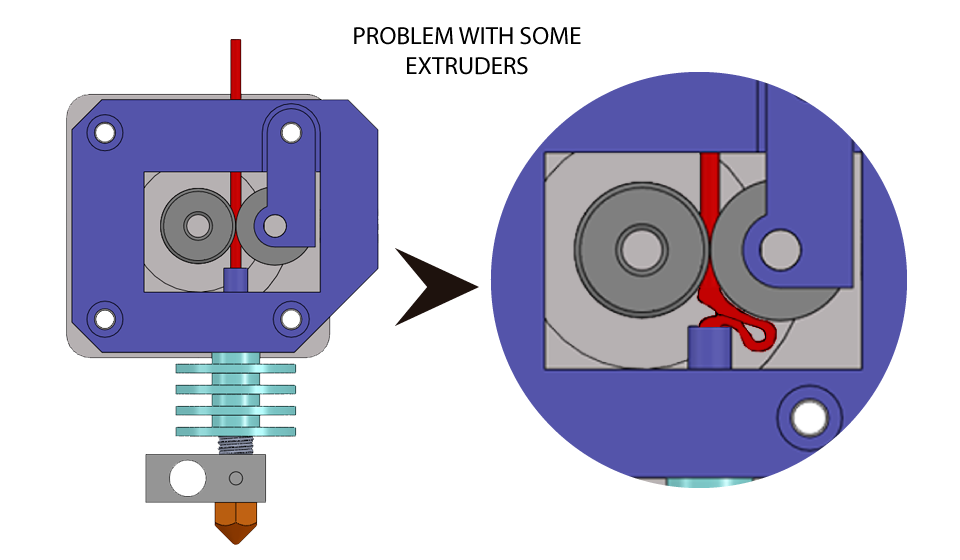
\includegraphics[width=0.5\textwidth,cfbox=azul_marcos 4pt 0pt]{FOTOS/NUDOS1}
\caption*{Extrudeuse NON optimisée pour l'impression de filaments flexibles}
\end{figure}
Ce problème est plus grand lorsqu'on utilise le filament de 1,75 mm puisqu’en ayant moins de section il risque de s'éloigner d’avantage de son itinéraire.
\\\\
La vitesse d’extrusion est déterminante pour l’apparition de ce problème. Si l’extrudeuse essaie de pousser le filament à la vitesse maximale, une pression vers le haut est créée poussant le filament à s’éloigner  de sa voie normale. C’est pour cela qu’on recommande généralement de lancer l’impression à une vitesse lente ou très lente et augmenter jusqu'à atteindre la vitesse maximale supportée par votre extrudeuse. La taille de la buse affecte aussi la limite de la vitesse maximale, plus elle est grande, plus le matériau fondu sera extrudé par unité de temps, et par conséquent, plus la vitesse à laquelle il est fait sera élevée.
\\\\
Les extrudeuses conçues pour utiliser des filaments souples minimisent les lacunes poussant le filament  à s’éloigner de sa voie  et elles incluent un système de double engrenage d’entraînement pour  enchaîner avec précision le filament et éviter complètement le problème en question, en même temps elles permettent d’augmenter la vitesse d’impression.
\begin{figure}[H]
\centering
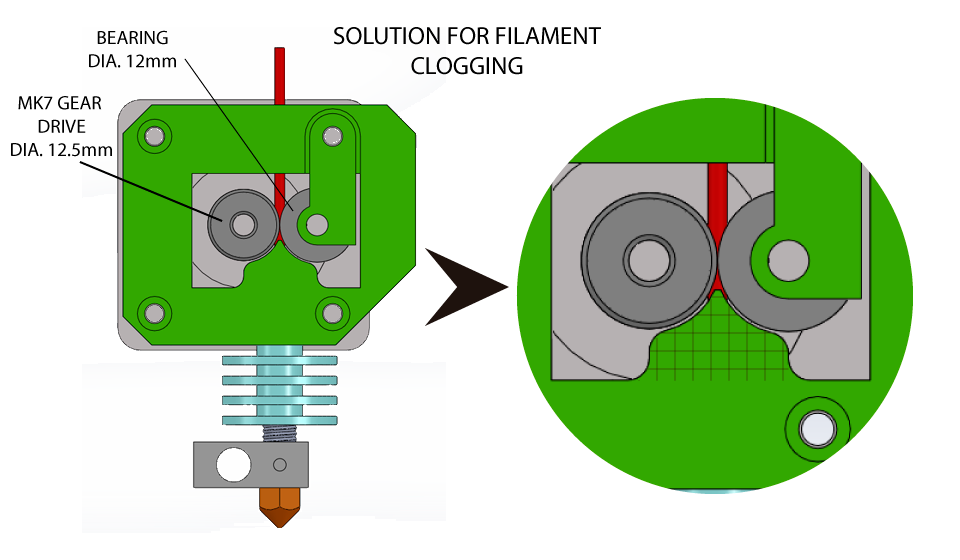
\includegraphics[width=0.5\textwidth,cfbox=azul_marcos 4pt 0pt]{FOTOS/NUDOS2}
\caption*{Extrudeuse optimisée pour l’impression de filaments souples}
\end{figure}
\emph{FlexiSMART a été conçu en tenant compte de ces problèmes ,il possède une rigidité supérieure à celles des autres filaments flexibles, pour aider à les minimiser.}
\\\\
Cependant, ces problèmes peuvent apparaître. Pour les extrudeuses qui ne sont pas conçues pour utiliser des matériaux élastiques.
	\subsection{Préparation de l'extrudeuse pour imprimer FlexiSMART}Si vous rencontrez des problèmes mentionnés précédemment vous avez probablement besoin de régler ou de remplacer votre extrudeuse. A ce propos, il y a quelques options que nous détaillons ci-dessous.
		\subsubsection{Modifier votre extrudeuse}
Parfois, il est possible d'utiliser FlexiSMART sur des extrudeuses non optimisées en appliquant quelques modifications sur l'extrudeuse elle-même
\\\\
Si vous rencontrez des problèmes d’impression FlexiSMART, nous vous suggérons de suivre les conseils suivants, présentés par ordre de complexité.
			\paragraph{Déposer la conduite à travers laquelle le filament accède à l'extrémité chaude}\mbox{}\\\\
Si vous utilisez une extrudeuse avec un corps en plastique, comme les extrudeuses imprimables, nous vous recommandons d'essayer ce qui suit.
\\\\
Déposer légèrement les bords du trou juste sous l’engrenage d'entraînement, un trou à travers lequel le filament est enchainé à l'extrémité chaude. Cela permet d'éviter les frottements et les attelages qui peuvent provoquer les nœuds précédemment décrits.
\\\\
Il est peut être nécessaire de démonter la partie de l’extrudeuse afin d’appliquer cette opération.
			\paragraph{Insérer le tube Téflon dans l’extrudeuse}\mbox{}\\\\
Une deuxième option, plus compliquée mais plus efficace, consiste à insérer un tube téflon (PTFE) dans le trou indiqué. Cette technique permet également de réduire l’espace avec l’engrenage d’entraînement puisque ce tube peut se placer très près de celui-là. Vous pouvez même modifier l’entrée du tube téflon pour l’adapter à la forme de l’engrenage d’entraînement en laissant un minimum d’espace.
\\\\
En général, cette technique implique de percer l’extrudeuse pour permettre l’insertion du tube téflon mentionné. Ici vous pouvez voir quelques images du résultat:
\begin{figure}[H]
    \centering
    \begin{subfigure}[b]{0.3\textwidth}
        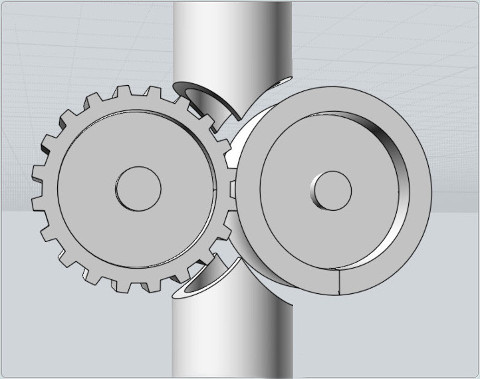
\includegraphics[width=\textwidth,cfbox=azul_marcos 4pt 0pt]{FOTOS/TEFLON1}
    \end{subfigure}
    ~ %add desired spacing between images, e. g. ~, \quad, \qquad, \hfill etc. 
      %(or a blank line to force the subfigure onto a new line)
    \begin{subfigure}[b]{0.3\textwidth}
        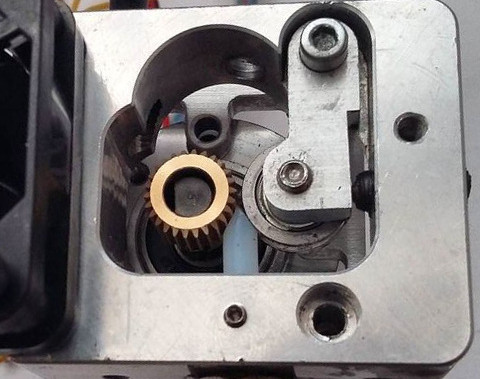
\includegraphics[width=\textwidth,cfbox=azul_marcos 4pt 0pt]{FOTOS/TEFLON2}
    \end{subfigure}
    ~ %add desired spacing between images, e. g. ~, \quad, \qquad, \hfill etc. 
    %(or a blank line to force the subfigure onto a new line)
    \begin{subfigure}[b]{0.3\textwidth}
        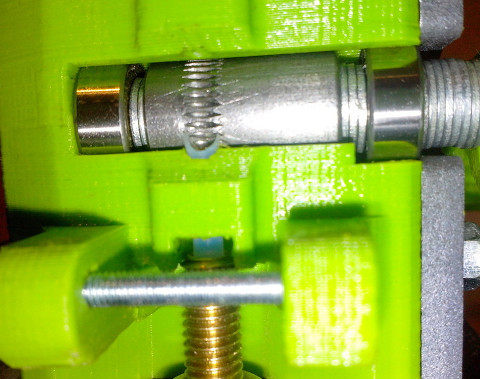
\includegraphics[width=\textwidth,cfbox=azul_marcos 4pt 0pt]{FOTOS/TEFLON3}
    \end{subfigure}
    \caption*{Insertions de tube (téflon) PTFE}
\end{figure}
			\paragraph{Imprimez un guide pour le filament et mettez-le dans l’extrudeuse}\mbox{}\\\\
Le troisième choix est d'imprimer une pièce qui sert de guide pour le filament et de la placer sous l’engrenage d’entraînement. Habituellement, ces pièces ont une forme triangulaire et devraient être conçues en respectant la dimension de chaque extrudeuse.
\\\\
Dans l’internet, dans des sites comme \url{www.thingiverse.com}, vous pouvez télécharger ce type de cartes pour certaines extrudeuses  les plus communes. Toutefois, il s’agit d’une conception simple permettant à ceux qui ont une connaissance de l’impression 3D de créer facilement et à partir de rien toutes pièces. 
\begin{figure}[H]
    \centering
    \begin{subfigure}[b]{0.5\textwidth}
        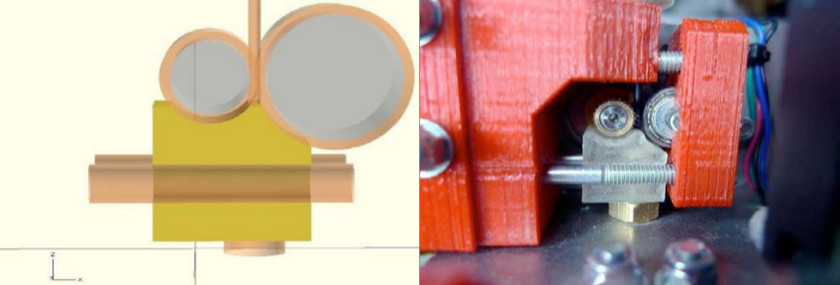
\includegraphics[width=\textwidth,cfbox=azul_marcos 4pt 0pt]{FOTOS/GUIA1}
    \end{subfigure}
    ~ %add desired spacing between images, e. g. ~, \quad, \qquad, \hfill etc. 
      %(or a blank line to force the subfigure onto a new line)
    \begin{subfigure}[b]{0.5\textwidth}
        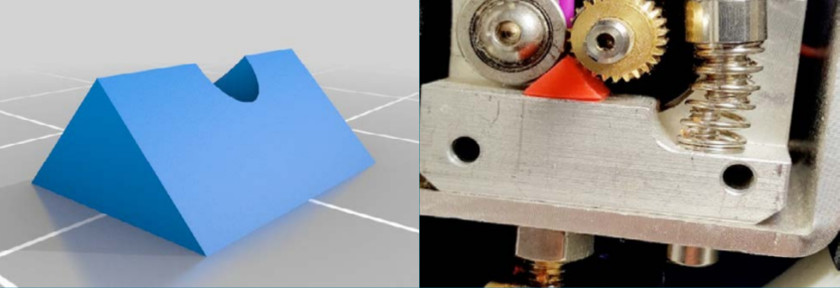
\includegraphics[width=\textwidth,cfbox=azul_marcos 4pt 0pt]{FOTOS/GUIA2}
    \end{subfigure}
    ~ %add desired spacing between images, e. g. ~, \quad, \qquad, \hfill etc. 
    %(or a blank line to force the subfigure onto a new line)
    \begin{subfigure}[b]{0.5\textwidth}
        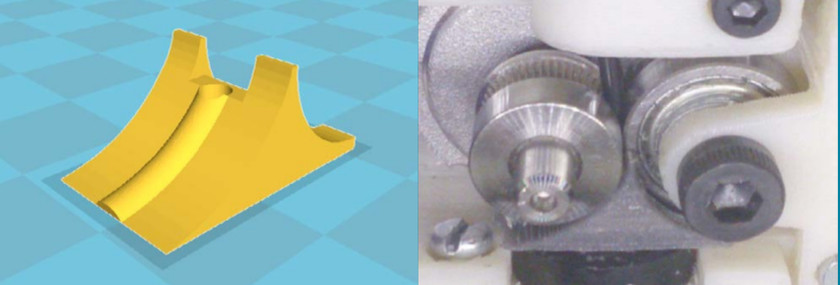
\includegraphics[width=\textwidth,cfbox=azul_marcos 4pt 0pt]{FOTOS/GUIA3}
    \end{subfigure}
    \caption*{Guides de filament imprimable}
\end{figure}	

	\paragraph{Réglage de pression de l’engrenage d’entraînement sur le filament}\mbox{}\\\\
Ceci étant un matériau souple, il est particulièrement important que la pression du mécanisme qui pousse le filament vers l'extrémité chaude ne soit pas excessive. Dans les filaments rigides, un excès de pression produira de petites entailles dans sa surface mais, dans le cas de FlexiSMART, une pression excessive déforme la section du filament, ce qui lui donnant une forme ovale qui le rend plus susceptible de boucher l'extrudeuse.
\\\\
Les extrudeuses conçus pour l’impression de filaments souples tiennent compte de ceci et ont un mécanisme pour régler la pression du mécanisme tracteur. Si votre extrudeuse permet de réguler cette pression, nous recommandons que vous l’ajuster en utilisant FlexiSMART. La pression adéquate sera le minimum nécessaire qui permet à l’extrudeuse de déplacer le filament.
\\\\
Si votre extrudeuse ne dispose pas d’un mécanisme permettant de régler la pression, vous pouvez le réduire encore en changeant le ressort ou en réduisant l’itinéraire éventuel en plaçant une cale au bon endroit. A titre d’exemple, nous présentons une image sur la façon de réduire la pression dans une extrudeuse qui n’est pas destinée pour cela :
\begin{figure}[H]
\centering
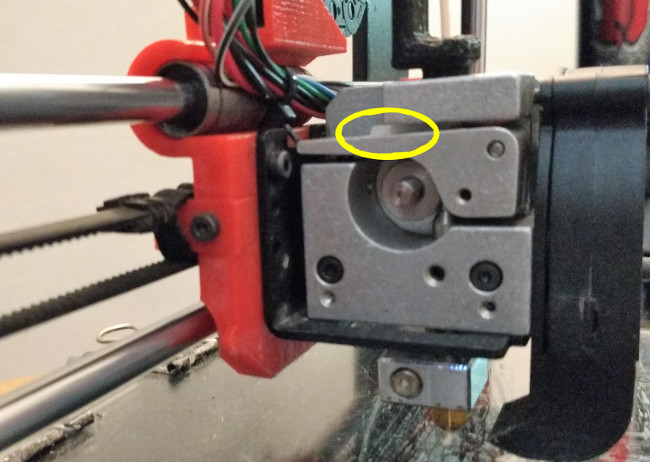
\includegraphics[width=0.5\textwidth,cfbox=azul_marcos 4pt 0pt]{FOTOS/SOLUCION1}
\caption*{HeatCore Extruder de BQ Hephestos y BQ Witbox}
\end{figure}
			\paragraph{Ajout de la tension entre la bobine et l'extrudeuse}\mbox{}\\\\
Il est prouvé que, dans certains modèles d’imprimantes, il est commode que lors de l’utilisation de filaments flexibles il y a lieu une certaine tension entre la bobine et l’extrudeuse de telle sorte que le filament ne soit pas suspendu.
\\\\
Pour obtenir ceci, vous pouvez essayer d’arrêter la bobine, afin que l’extrudeuse tire légèrement le filament à démêler. Vous pouvez également placer un accessoire similaire à celui de la photo pour atteindre la même cible.
\begin{figure}[H]
\centering
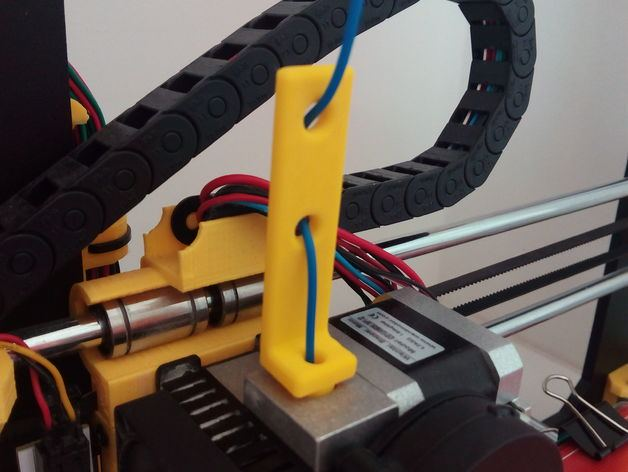
\includegraphics[width=0.5\textwidth,cfbox=azul_marcos 4pt 0pt]{FOTOS/SOLUCION2}
\caption*{BQ Unibody extruder}
\end{figure}
		\subsubsection{Remplacer votre extrudeuse par un optimisé}
De nos jours les filaments flexibles sont devenus populaires au point où il est devenu évident que l’imprimante de dernière génération soient disposée à les imprimer.
\\\\
En outre, beaucoup de concepteurs ont créé des extrudeuses imprimables capable d’imprimer les FlexiSMART et autres filaments. Ces extrudeuses peuvent être téléchargées depuis les pages comme Thingiverse à imprimer et assembler à la maison.
\\\\
Il y a aussi de plus en plus des extrudeuses commerciales disposées à imprimer des filaments souples qui peuvent être obtenues et montées sur nos imprimantes.
			\paragraph{DIY extrudeuses imprimables}\mbox{}\\\\
Certains de ces extrudeuses sont conçus à partir de rien et d’autres sont issues des modifications apportées au fil des conceptions existantes. Nous présentons ici une liste non exhaustive de conceptions de l’extrudeuse téléchargeable sur internet. Dans chaque lien, vous trouverez la liste complète des composants ainsi que les instructions de montage et les commentaires d’autres utilisateurs.
\\\\
Le bout chaud que vous installez sur votre extrudeuse doit avoir un tube téflon (PTFE) à l’intérieur pour éviter les frottements et ainsi que FlexiSMART peut s’ imprimée correctement. FlexiSMART a été testé avec succès sur le bout chaud suivant\footnote{Vous devez tenir en compte que les tests en question ont été réalisés avec des bouts chaud originaux et nous ne pouvons garantir le même résultat sur les imitations.}:
\begin{itemize}
\item J-Head MKV-B
\item Budassnozzle V1.3
\item E3D v6
\item Leonnozzle V2
\end{itemize}
Selon quelle imprimante que vous utilisez, certaines extrudeuses seront plus faciles à installer, étant donné qu’elles pourraient remplacer l’extrudeuse original de la machine.
\begin{figure}[H]
    \centering
    \begin{subfigure}[b]{0.4\textwidth}
        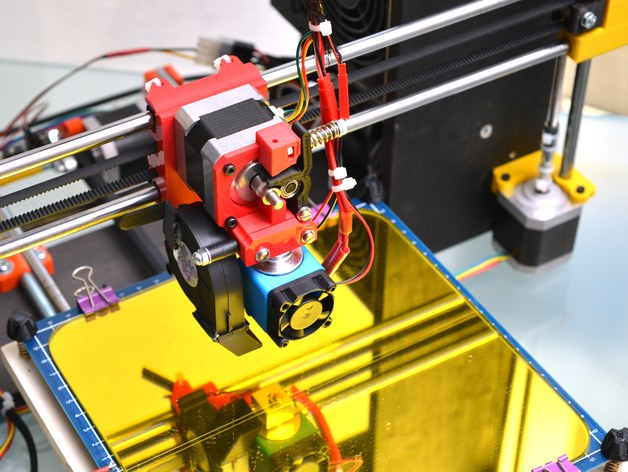
\includegraphics[width=\textwidth,cfbox=azul_marcos 4pt 0pt]{FOTOS/EXTRUSOR1}
		\caption*{\href{http://www.thingiverse.com/thing:147705}{{\footnotesize Direct-drive hinged extruder for E3D/J-Head hot-end (Prusa i3) by ffleury}}}
    \end{subfigure}
    ~ \qquad%add desired spacing between images, e. g. ~, \quad, \qquad, \hfill etc. 
      %(or a blank line to force the subfigure onto a new line)
    \begin{subfigure}[b]{0.4\textwidth}
        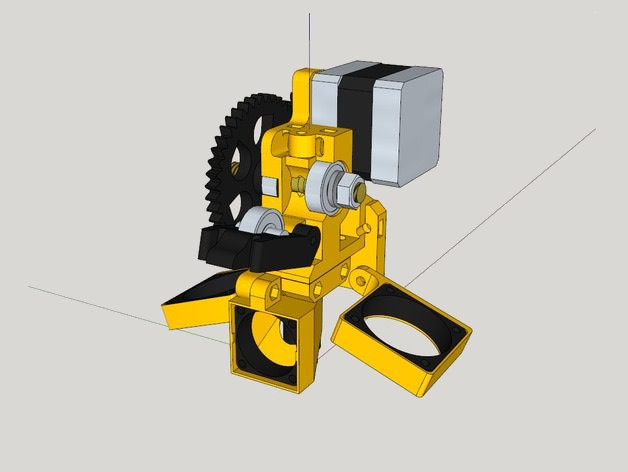
\includegraphics[width=\textwidth,cfbox=azul_marcos 4pt 0pt]{FOTOS/EXTRUSOR2}
		\caption*{\href{http://www.thingiverse.com/thing:512338}{{\footnotesize Wade L3K Extruder (prusa I3) compatible filament flexible By Skarab}}}
    \end{subfigure}
\end{figure}
\begin{figure}[H]
    \centering
    ~ %add desired spacing between images, e. g. ~, \quad, \qquad, \hfill etc. 
    %(or a blank line to force the subfigure onto a new line)
    \begin{subfigure}[b]{0.4\textwidth}
        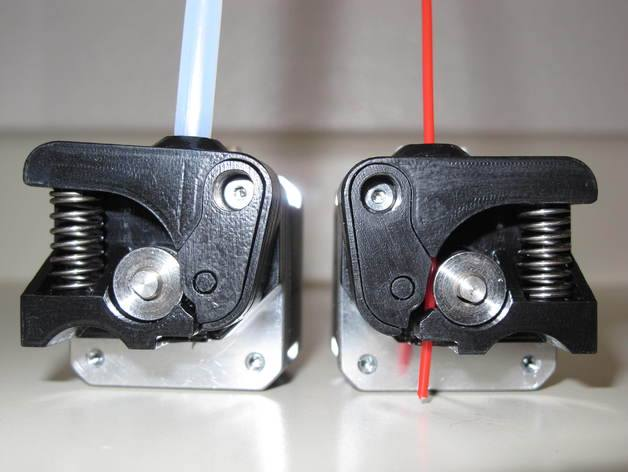
\includegraphics[width=\textwidth,cfbox=azul_marcos 4pt 0pt]{FOTOS/EXTRUSOR3}
		\caption*{\href{http://www.thingiverse.com/thing:403438}{{\footnotesize Printrbot Flexible Filament Direct Drive Extruder by thirdhorizon}}}
    \end{subfigure}
    ~ \qquad %add desired spacing between images, e. g. ~, \quad, \qquad, \hfill etc. 
    %(or a blank line to force the subfigure onto a new line)
    \begin{subfigure}[b]{0.4\textwidth}
        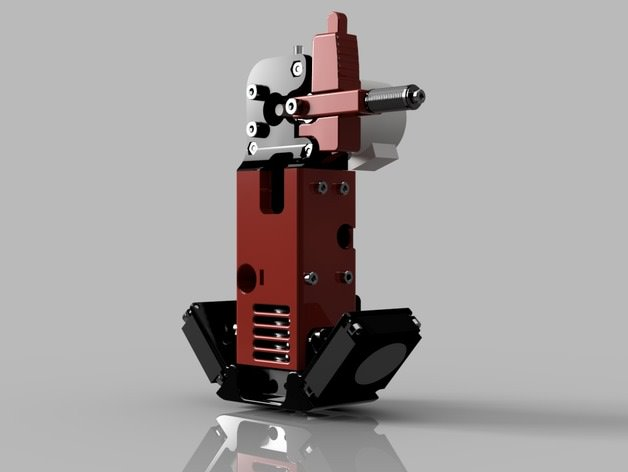
\includegraphics[width=\textwidth,cfbox=azul_marcos 4pt 0pt]{FOTOS/EXTRUSOR4}
		\caption*{\href{http://www.thingiverse.com/thing:1102900}{{\footnotesize Ultimaker 2 PG35L Direct Drive Extruder for 1.75mm E3D v6 Hotend by jasonatepaint}}}
    \end{subfigure}
\end{figure}
			\paragraph{Extrudeuses commerciales}\mbox{}\\\\
L’acquisition d’une extrudeuse commerciale est plus cher que sa construction à la maison, par contre, elle a habituellement une performance meilleur que cette dernière et elle demeure le meilleur choix au cas où vous envisagez une utilisation  intensive des filament flexible.
\\\\
Ces extrudeuses ont été spécifiquement conçues pour éviter tous les problèmes mentionnés précédemment, et certaines peuvent extruder FlexiSMART à des vitesses supérieures à 70 mm/s.
\begin{figure}[H]
    \centering
    \begin{subfigure}[b]{0.4\textwidth}
        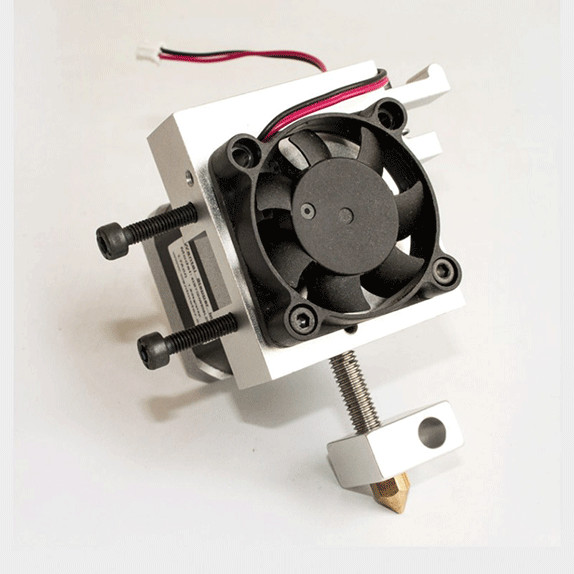
\includegraphics[width=\textwidth,cfbox=azul_marcos 4pt 0pt]{FOTOS/EXTRUSOR5}
		\caption*{\href{http://www.recreus.com}{{\footnotesize Recreus Extruder - Precio aprox. 100\euro}}}
    \end{subfigure}
    ~ \qquad%add desired spacing between images, e. g. ~, \quad, \qquad, \hfill etc. 
      %(or a blank line to force the subfigure onto a new line)
    \begin{subfigure}[b]{0.4\textwidth}
        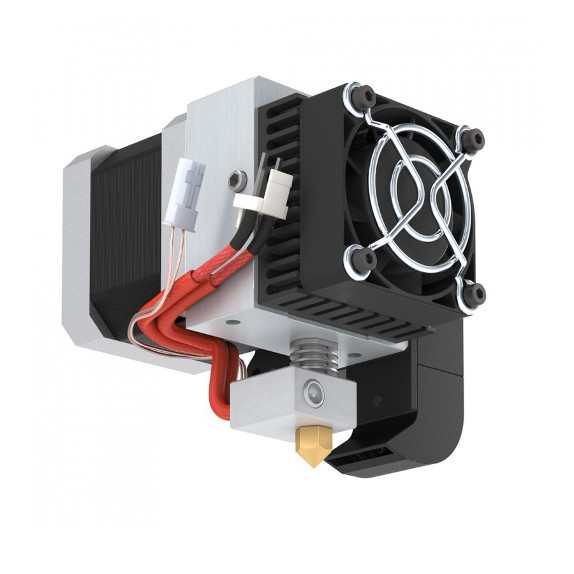
\includegraphics[width=\textwidth,cfbox=azul_marcos 4pt 0pt]{FOTOS/EXTRUSOR6}
		\caption*{\href{http://www.bq.es}{{\footnotesize BQ HeatCore DDG Extruder - Precio 140\euro}}}
    \end{subfigure}
\end{figure}
\begin{figure}[H]
    \centering
    ~ %add desired spacing between images, e. g. ~, \quad, \qquad, \hfill etc. 
    %(or a blank line to force the subfigure onto a new line)
    \begin{subfigure}[b]{0.4\textwidth}
        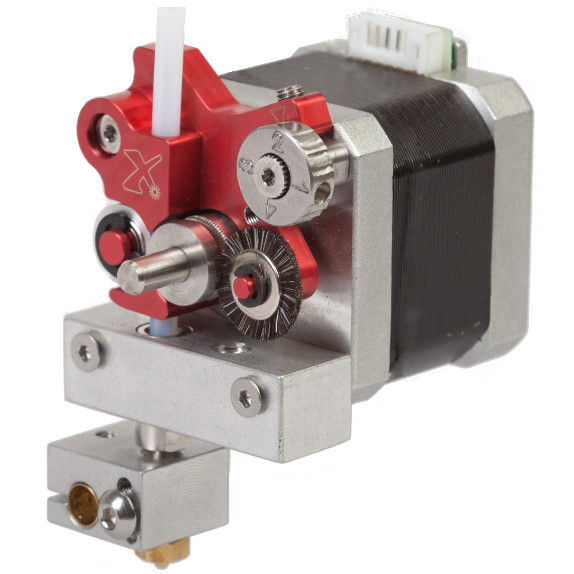
\includegraphics[width=\textwidth,cfbox=azul_marcos 4pt 0pt]{FOTOS/EXTRUSOR7}
		\caption*{\href{https://flexionextruder.com/}{{\footnotesize Flexion Extruder - Precio aprox. 140\euro}}}
    \end{subfigure}
    ~ \qquad %add desired spacing between images, e. g. ~, \quad, \qquad, \hfill etc. 
    %(or a blank line to force the subfigure onto a new line)
    \begin{subfigure}[b]{0.4\textwidth}
        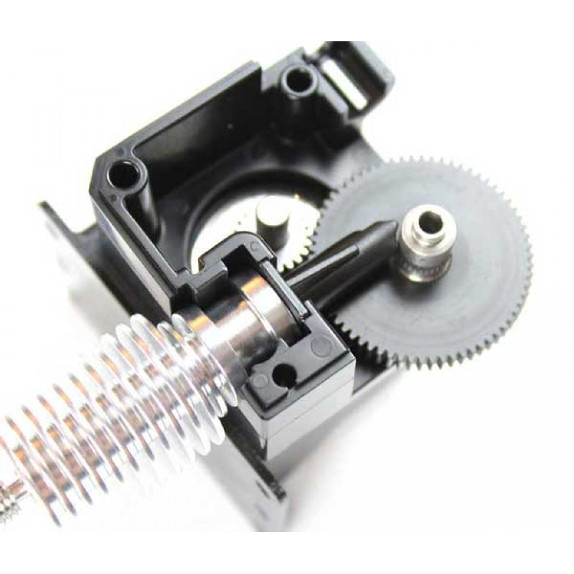
\includegraphics[width=\textwidth,cfbox=azul_marcos 4pt 0pt]{FOTOS/EXTRUSOR8}
		\caption*{\href{www.e3d-online.com}{{\footnotesize Titan Extruder - Precio aprox. 70\euro}}}
    \end{subfigure}
\end{figure}
\section{Conseils pour une utilisation optimale des FlexiSMART}
	\subsection{Rétraction}
La rétraction est une technique utilisée sur les imprimantes 3D FFF / FDM pour améliorer la finition des pièces imprimées. Elle consiste à commander à l'extrudeuse de retirer quelques centimètres du filament lorsque celui-ci est sur le point de changer de position pour éviter le cordage ou l'apparition de petits fils de filament sur différentes parties de la pièce en cours d'impression.
\begin{figure}[H]
\centering
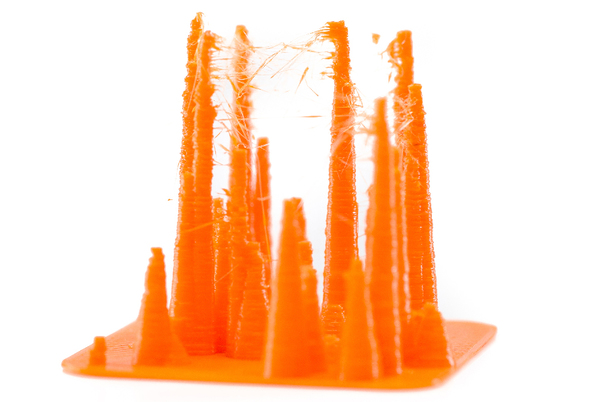
\includegraphics[width=0.5\textwidth,cfbox=azul_marcos 4pt 0pt]{FOTOS/RETRACCION1}
\caption*{Une pièce avec problèmes de cordage}
\end{figure}
Lors de l’utilisation de filaments flexibles, il peut y arriver qu’en essayant de faire une rétractation très brusque, le filament s'étire au lieu de se retirer. C’est pourquoi il est très recommandé d’utiliser des paramètres de rétraction différents de ceux utilisés avec des filaments rigides.
\\\\
Les 2 paramètres que nous pouvons contrôler dans la rétraction sont la taille, ou la valeur linéaire en millimètres du filament rétracté et la vitesse de l’opération  mm/s. Les deux valeurs doivent être inférieurs à celles utilisées régulièrement. Le meilleur moyen de calibrer ces valeurs consiste à exécuter des tests pour déterminer  les valeurs maximales de votre imprimante peuvent être prise en compte lors de l’impression avec FlexiSMART. Dans tous  cas, comme point de départ, vous pouvez utiliser les valeurs que nous recommandons:
\begin{description}
\item [Taille de rétraction:] 1.5 mm
\item [Vitesse de rétraction:] 40 mm/s
\end{description}
En Fonction de l’imprimante, il peut s’avérer nécessaire de désactiver complètement la rétraction.
	\subsection{Impression séquentielle}
FlexiSMART et autres filaments souples ont une viscosité différente à celle des autres matériaux lorsqu’il atteint sa température de fusion. Pour cela, il est plus évident de de laisser les petits fils de filament entre les différentes parties de la pièce lorsque la buse doit se déplacer d’un point à l’autre sans extrusion.
\begin{figure}[H]
\centering
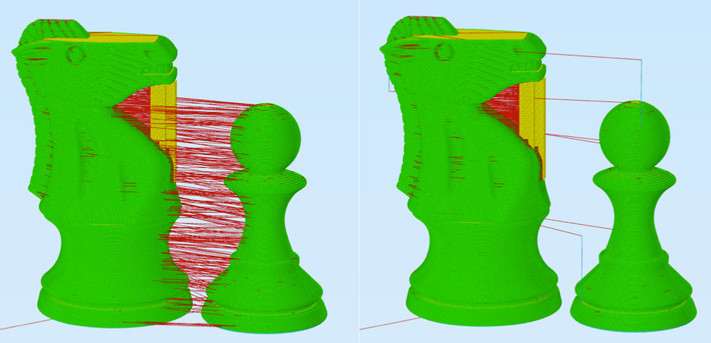
\includegraphics[width=0.5\textwidth,cfbox=azul_marcos 4pt 0pt]{FOTOS/SEQUENTIALPRINTING}
\caption*{Comparaison entre les modes d'impression simultanés et séquentiels}
\end{figure}
D’ailleurs, lorsque plusieurs pièces vont être imprimées en même temps, ces petits filets peuvent apparaître entre les pièces puisque la buse doit sauter constamment de l'un à l'autre.
\\\\
Comme nous l'avons déjà mentionné, cet effet peut se réduire à l’aide de rétraction, mais il est fortement recommandé que les différentes pièces soient imprimées séquentiellement au lieu d’être imprimées simultanément.
\\\\
Nous entendons, par séquentiel l’impression complète de la pièce avant de commencer l’impression de la suivante.
\\\\
Ceci est réalisable selon deux manières différentes :
\begin{itemize}
\item L'option triviale est d'imprimer une seule pièce et une fois terminée répéter la même impression autant de fois que voulu.
\item La deuxième alternative, plus avancée et avec certaines limites, consiste à utiliser l'option de stratification que certains programmes proposent, au lieu d'imprimer une pièce à la fois. Vous optez pour La taille maximale des pièces imprimable. En utilisant cette méthode vous dépendrez des dimensions de la buse et la disposition de l'axe de l'imprimante. Nous vous recommandons vivement d'obtenir des informations sur la façon d’utiliser ces options pour ne pas courir le risque d’endommager votre imprimante. Nous vous invitons à vous informer concernant cela à travers les liens suivants:
\end{itemize}
\url{https://www.simplify3d.com/support/tutorials/multi-part-printing/}\\
\url{http://manual.slic3r.org/advanced/sequential-printing}\\
\url{https://ultimaker.com/en/community/3843-force-cura-to-print-objects-separately}
	\subsection{La première couche}
La première couche est la base des couches suivantes et elle marque la différence entre un une impression satisfaisant et une impression ratée.
\\\\
Lors de l’impression avec FlexiSMART il faut bien faire une attention en particulier à la première couche car, parfois, une imprimante correctement nivelée pour imprimer avec PLA ou ABS, ne l’est pas forcement avec FlexiSMART pour imprimer adéquatement.
\\\\
Pour savoir si l'imprimante est correctement nivelée, vous devrez regarder attentivement comment la machine fabrique la première couche.
\\\\
Si la première couche semble translucide, cela signifie que la buse est trop proche de la plate-forme et qu’il serait nécessaire de la séparer de quelques microns.
\\\\
En revanche, si la première couche semble se détacher ou les pistes du matériau déposées montrent des espaces sans plastique entre eux, il serait nécessaire d’approcher la buse de quelques microns de la plate-forme.
\begin{figure}[H]
    \centering
    \begin{subfigure}[b]{0.3\textwidth}
        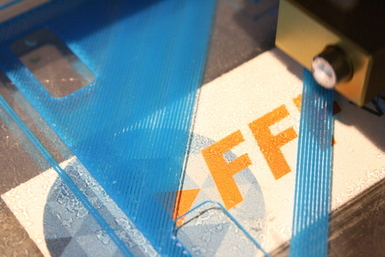
\includegraphics[width=\textwidth,cfbox=azul_marcos 3pt 0pt]{FOTOS/HOTENDALTO}
	\caption*{Buse trop loin}
    \end{subfigure}
    ~ %add desired spacing between images, e. g. ~, \quad, \qquad, \hfill etc. 
      %(or a blank line to force the subfigure onto a new line)
    \begin{subfigure}[b]{0.3\textwidth}
        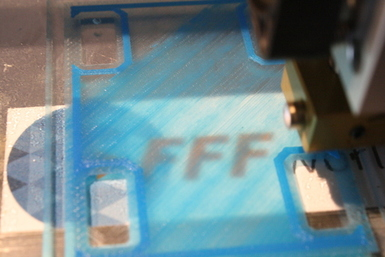
\includegraphics[width=\textwidth,cfbox=azul_marcos 3pt 0pt]{FOTOS/HOTENDBAJO}
	\caption*{Buse trop près}
    \end{subfigure}
    ~ %add desired spacing between images, e. g. ~, \quad, \qquad, \hfill etc. 
    %(or a blank line to force the subfigure onto a new line)
    \begin{subfigure}[b]{0.3\textwidth}
        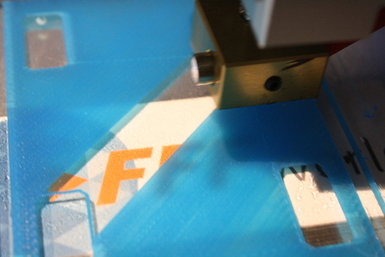
\includegraphics[width=\textwidth,cfbox=azul_marcos 3pt 0pt]{FOTOS/HOTENDPERFECTO}
	\caption*{Buse bien nivelé}
    \end{subfigure}
\end{figure}
Cet ajustement peut se faire par logiciel, réglage de l’offset-z dans le programme de stratification ou régler le mécanisme de niveau de la plate-forme d’impression.
	\subsection{Conseils de stratification}
		\subsubsection{La hauteur de la couche}
La hauteur de la couche détermine la qualité de la ièce et le temps d’impression.
\\\\
À l’aide d’une buse de 0.4 mm nous avons prouvé que la hauteur optimale de la couche est de 0,2 mm. Avec cette hauteur de la couche, vous obtiendrez des couches fortement attachées avec une excellente finition de surface.
		\subsubsection{Les couches supérieures et les périmètres}
Les couches supérieures et les périmètres sont l’habillage latéral et supérieur de la pièce.
\\\\
Le nombre suffisant entre elles dépendra du remplissage et de l’usage destiné à la pièce.
\\\\
Avec un remplissage élevé, vous pouvez réduire le nombre de couches supérieures à 3 puisque le remplissage de la pièce leur donnera une bonne base pour bien se positionner. En optant pour quelques valeurs moyennes ou faibles de remplissage il est recommandée d’ augmenter le nombre de couches supérieures à 5 afin de s'assurer que la partie supérieure de la pièce est complètement étanche.
\\\\
Si la pièce risque de subir des déformations, il est recommandé d’augmenter le nombre de coquilles ou de périmètres horizontaux. L'augmentation du nombre de périmètres horizontaux exerce une pression ou traction sur les parois de la pièce pour l’arrêter sans qu’elle dépasse le logement.
\\\\
Ces recommandations sont valables lorsque vous utilisez une buse de 0,4 mm et une hauteur de couche de 0,2 mm. Si la taille de la buse ou de la couche varie, le nombre optimale de périmètres et des couches supérieures changeront également.
\\\\
Nous vous invitons lancer vos propres tests et de partager les résultats avec nous.
		\subsubsection{Influence du remplissage sur la flexibilité}
Le taux et la conception du remplissage a une grande influence sur le degré de flexibilité des pièces imprimées avec FlexiSMART.
\\\\
Une pièce avec un remplissage près de 100\% se comportera comme un bloc de caoutchouc et peut être un bon choix pour les pièces telles que des silent-blocs ou des entretoises.
\\\\
En optant pour un remplissage de 15\%, vous obtiendrez des pièces molles qui risquent de s’e écraser et se déformer.
\\\\
Le modèle de remplissage affecte également la flexibilité et un remplissage rectiligne ne se comporte pas comme un remplissage en nid d'abeille. Nous vous invitons à faire vos propres tests et à choisir celui qui vous convient le mieux.
	\subsection{Utilisation d’une buse de taille supérieure}
La buse standard de la plupart des imprimantes a 0,4 mm, une taille de la buse qui donne un ratio de bonne vitesse/résolution. FlexiSMART s’imprime parfaitement avec ce type de buse, toutefois, il convient d’apporter quelques précisions.
\\\\
La taille de la buse limite la quantité de matière qu’on peut extruder par unité de temps. À l’aide de filaments rigides, cette limite est plus élevée d’autant que la vitesse peut augmenter et que le filament lui-même supporte la pression supplémentaire nécessaire pour la sortie du matériel à par la buse. Cependant Avec FlexiSMART, le filament est compressé si cette pression est trop élevée et qu’en règle générale, il doit être imprimé à basse vitesse.
\\\\
Donc si vous voulez extruder FlexiSMART à des vitesses élevées, ‘il est recommandé d’ utiliser une buse de plus grande taille, de 0,6 mm. en utilisant l’une de ces buses vous pouvez imprimer beaucoup plus rapidement, avec plus de hauteurs pour la couche supérieure, tout en sacrifiant une certaine résolution.
\section{Souhaitez-vous soutenir notre projet?}
Tous les membres de FFF monde aiment impression 3D et la communauté de la machine. Nous nous estimons chanceux d’être en mesure de travailler sur des projets où nous pouvons vous livrer honnêtement notre passion. À l’avenir, nous aimerions être en mesure de développer plus de matériaux, plus de couleurs et plus de formats. En fin de compte, nous aimerions faire grandir notre entreprise.
\\\\
Par conséquent, une des meilleures actions pour nous aider, si vous le souhaitez et que vous êtes satisfait du filament, est de nous donner 5 étoiles sur Amazon.
\begin{figure}[H]
\centering

\includegraphics[width=0.5\textwidth,cfbox=azul_marcos 1pt 0pt]{FOTOS/AMAZON_FIVE_STARS}
\caption*{Merci beaucoup!}
\end{figure}
\subsection{Autres filaments avec propriétés génial aujourd'hui disponibles dans Amazon}
\begin{description}
  \item[FlexiSMART Tech:] Conçu pour résister à l’abrasion et l’usure des impressions techniques.
\item[ABS Tech:] Effet déformation réduit. Hautes performances sur les applications techniques.
\item[PETG Tech:] Résistance mécanique maximale. Résistance au contact avec l’eau et les rayons UV. Aptitude pour usage alimentaire.
\item[FilaMETAL:] PLA avec une charge métallique non abrasive qui donne une finition mécanique spectaculaire à vos impressions.
\item[PC Tech:] Polycarbonates offrant une résistance élevée à la température et excellentes propriétés mécaniques.
\item[Nylon Tech:] Imprimable à basse température. Résistance aux coups avec un certain degré de flexibilité.
\item[PVA Tech:] Filament soluble dans l’eau destiné pour servir de matériau de support. Excellente compatibilité avec PLA.
\item[HIPS Tech:] Filament soluble dans le Limonène destiné pour servir de matériau de support. Bonne résistance mécanique et excellente compatibilité avec l'ABS.
\end{description}
%\section{Bibliografía}
%Esta guía no habría sido posible sin el conocimiento libre generado por la comunidad RepRap. Para la elaboración de esta guía se han %utilizado imágenes y contenido extraidos de los siguientes sitios web.
%\\\\
%\url{http://www.gyrobot.co.uk/blog/how-to-3d-print-with-flexible-filaments}\\
%\url{http://www.thingiverse.com/thing:1496895}\\
%\url{http://www.thingiverse.com/thing:247024}\\
%\url{http://www.thingiverse.com/thing:16319}\\
%\url{http://www.thingiverse.com/thing:779011}\\
%\url{http://www.thingiverse.com/thing:1102900}\\
%\url{http://www.thingiverse.com/thing:147705}\\
%\url{http://www.thingiverse.com/thing:222667}\\
%\url{http://www.thingiverse.com/thing:512338}\\
%\url{https://all3dp.com/common-3d-printing-problems-and-their-solutions/}\\
%\url{https://www.simplify3d.com/support/}\\
%\url{http://www.thingiverse.com/thing:508896}\\
%\url{http://www.thingiverse.com/thing:1187344}

\includepdf{PDF/FR_CONTRAPORTADA.pdf}
\end{document}
